\section{Kalman Filter for prediction}

Let's examine a straightforward system devoid of external influences, characterized by linearity and time-invariance.

\subsection{System description}
We're dealing with a multiple input multiple output system denoted as $\mathcal{S}$, described by the following equations:
\[\mathcal{S}:\begin{cases}
    \mathbf{x}(t+1)=\mathbf{Fx}(t)+\mathbf{Gu}(t)+\mathbf{v}_1(t) \\
    \mathbf{y}(t)=\mathbf{Hx}(t)+\mathbf{Du}(t)+\mathbf{v}_2(t)
\end{cases}\]
In this configuration, there are $n$ states, $p$ inputs, and $m$ outputs. 

\paragraph*{First White Noise}
The vector White Noise $\mathbf{v_1}(t)$ characterizes internal disturbances and minor model inaccuracies, with zero mean and variance $V_1$:
\[\mathbf{v}_1(t)=\begin{bmatrix} v_{11}(t) \\ v_{12}(t) \\ \vdots \\ v_{1n}(t) \end{bmatrix}\]
It's termed model noise. 
Its properties are:
\begin{enumerate}
    \item Each element of the $\mathbf{v}_1(t)$ matrix has an expected value of zero:
        \[\mathbb{E}\left[\mathbf{v}_1(t)\right]=0\]
    \item The covariance matrix of $\mathbf{v}_1(t)$ is determined as:
        \[V_1=\mathbb{E}\left[\mathbf{v}_1(t)\mathbf{v}_1(t)^T\right]\]
        This matrix is square, symmetric, and positive semi-definite.
    \item Covariance is zero:
        \[\mathbb{E}\left[\mathbf{v}_1(t)\mathbf{v}_1(t-\tau)^T\right]=0\qquad \forall t, \forall\tau\neq 0\]
\end{enumerate}

\paragraph*{Second White Noise}
The vector White Noise $\mathbf{v}_2(t)$ characterizes internal disturbances and minor model inaccuracies, with zero mean and variance $V_2$:
\[\mathbf{v}_2(t)=\begin{bmatrix} v_{21}(t) \\ v_{22}(t) \\ \vdots \\ v_{2p}(t) \end{bmatrix}\]
It's termed sensor noise. 
Its properties are:
\begin{enumerate}
    \item Each element of the $\mathbf{v}_2(t)$ matrix has an expected value of zero:
        \[\mathbb{E}\left[\mathbf{v}_2(t)\right]=0\]
    \item The covariance matrix of $\mathbf{v}_2(t)$ is determined as:
        \[V_2=\mathbb{E}\left[\mathbf{v}_2(t)\mathbf{v}_2(t)^T\right]\]
        This matrix is square, symmetric, and assumed to be positive definite, a requirement for applications involving the Differential Riccati Equation.
    \item Covariance is zero:
        \[\mathbb{E}\left[\mathbf{v}_2(t)\mathbf{v}_2(t-\tau)^T\right]=0\qquad \forall t, \forall\tau\neq 0\]
\end{enumerate}

\paragraph*{Assumptions}
Given the dynamical nature of the system, certain assumptions about initial conditions are necessary. 
We assume that:
\begin{itemize}
    \item The expected value of the initial state $\mathbf{x}(1)$ is $\mathbf{x}_0$: 
        \[\mathbb{E}\left[\mathbf{x}(1)\right]=\mathbf{x}_0\]
    \item The expected value of the outer product of the difference between the initial state and $x_0$ with its transpose is $P_0$, where $P_0$ is non-negative: 
        \[\mathbb{E}\left[\left(\mathbf{x}(1)-\mathbf{x}_0\right)\left(\mathbf{x}(1)-\mathbf{x}_0^T\right)\right]=\mathbf{P}_0\geq 0\]
\end{itemize}
This approach provides a probabilistic description of the initial state, encompassing both its mean value and variance.
If $\mathbf{P}_0=0$, it implies precise knowledge of the initial state.

\paragraph*{Correlation between the two White Noises}
We make the assumption that the correlation between $\mathbf{v}_1(t)$ and $\mathbf{v}_2(t-\tau)$ is given by:
\[\mathbb{E}=\left[\mathbf{v}_1(t)\mathbf{v}_2(t-\tau)^T\right]=\begin{cases}
    0 \qquad\quad\text{if }\tau\neq 0 \\
    V_{12} \qquad\:\text{if }\tau= 0
\end{cases}\]
Typically, $V_{12}=0$.

\paragraph*{Correlation between the White Noises and the initial state}
It's assumed that both White Noises $\mathbf{v}_1(t)$ and $\mathbf{v}_2(t)$ are uncorrelated with the initial state $\mathbf{x}(1)$. 
This technical assumption ensures the theoretical optimality of the Kalman Filter.

\subsection{One step predictor}
We utilize the following solution:
\[\begin{cases}
    \hat{\mathbf{x}}(t+1\mid t)=\mathbf{F}\hat{\mathbf{x}}(t\mid t-1)+\mathbf{K}(t)\mathbf{e}(t) \\ 
    \hat{\mathbf{y}}(t+1\mid t)=\mathbf{H}\hat{\mathbf{x}}(t\mid t-1) \\
    \mathbf{e}(t)=\mathbf{y}(t)-\hat{\mathbf{y}}(t\mid t-1) \\
    \mathbf{K}(t)=\left(\mathbf{FP}(t)\mathbf{H}^T+V_{12}\right)\left(\mathbf{HP}(t)\mathbf{H}^T+V_2\right)^{-1} \\
    \mathbf{P}(t+1)=\left(\mathbf{FP}(t)\mathbf{F}^T+V_1\right)-\left(\mathbf{FP}(t)\mathbf{H}^T+V_{12}\right)\left(\mathbf{HP}(t)\mathbf{H}^T+V_{2}\right)^{-1}\left(\mathbf{FP}(t)\mathbf{H}^T+V_{12}\right)^T
\end{cases}\]
Each equation serves a distinct purpose:
\begin{enumerate}
    \item \textit{State equation}: predicts the next state based on the current state and the system's dynamics.
    \item \textit{Output equation}: predicts the next output based on the predicted state.
    \item \textit{Error equation}: computes the prediction error between the actual output and the predicted output.
    \item \textit{Gain equation}: computes the optimal Kalman gain.
    \item \textit{Differential Riccati Equation}: computes the covariance matrix of the one-step prediction error of the states.
\end{enumerate}
To ensure the solution's validity, we require initial conditions:
\[\begin{cases}
    \hat{\mathbf{x}}(1\mid 0)=\mathbf{x}_0 \\
    \mathbf{P}(1)=\mathbf{P}_0
\end{cases}\]

\paragraph*{Differential Riccati Equation and gain structure}
The structure of $\mathbf{K}(t)$ and the Differential Riccati Equation  is block-wise. 
The three essential blocks involved are:
\begin{itemize}
    \item State block: $\mathbf{FP}(t)\mathbf{F}^T+V_1$.
    \item Output block: $\mathbf{HP}(t)\mathbf{H}^T+V_{2}$.
    \item Mix block: $\mathbf{FP}(t)\mathbf{H}^T+V_{12}$.
\end{itemize}

\paragraph*{Differential Riccati Equation}
The Differential Riccati Equation a specialized type of nonlinear matrix difference equation. 
It represents an autonomous system devoid of inputs:
\[\begin{cases}
    \mathbf{P}(t+1)=f(\mathbf{P}(t)) \\
    \mathbf{P}(1)=\mathbf{P}_0
\end{cases}\]
To ensure the existence of the Differential Riccati Equation at all time instants, $\mathbf{HP}(t)\mathbf{H}^T+V_2$ must be invertible. 
Given our assumption that $V_2$ is positive semi-definite, the full matrix becomes positive definite and thus invertible.

\paragraph*{Prediction error}
The matrix $\mathbf{P}(t)$ is a symmetric $n \times n$  matrix representing the covariance matrix of the one-step prediction error of the states:
\[\mathbf{P}(t)=\mathbb{E}\left[\left(\mathbf{x}(t)-\hat{\mathbf{x}}(t\mid t-1)\right)\left(\mathbf{x}(t)-\hat{\mathbf{x}}(t\mid t-1)\right)^T\right]=\text{Var}\left[\mathbf{x}(t)-\hat{\mathbf{x}}(t\mid t-1)\right]\]

\paragraph*{Graphical representation}
The block diagram of the system and the Kalman Filter is depicted below:
\begin{figure}[H]
    \centering
    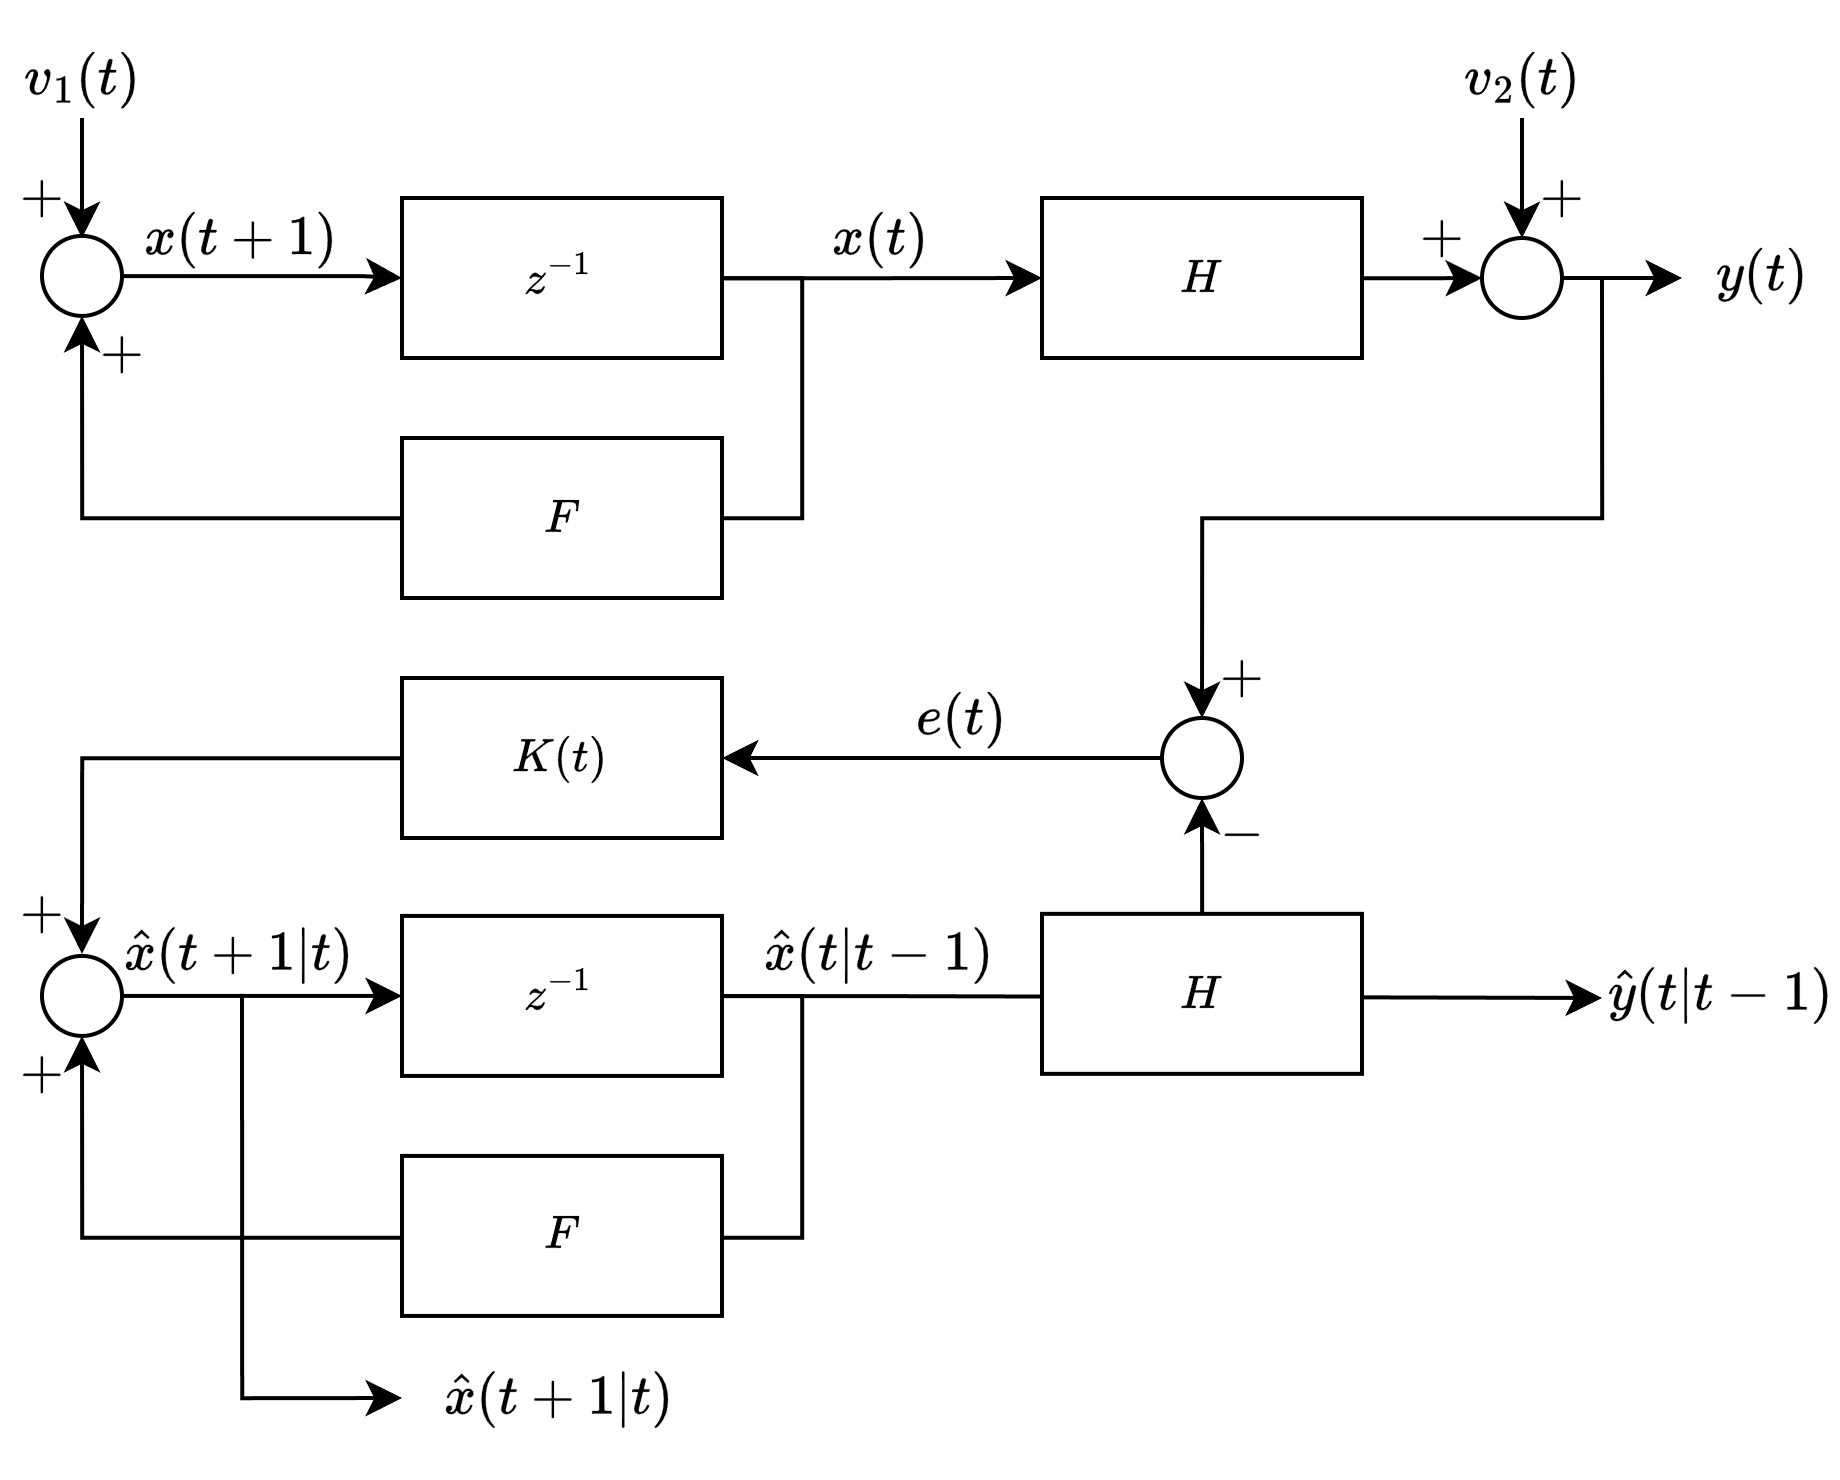
\includegraphics[width=0.75\linewidth]{images/kalman.png}
\end{figure}
The structure of the Kalman Filter is straightforward and intuitive:
\begin{itemize}
    \item It mimics the system's structure, excluding the two unmeasurable noises.
    \item It computes the real output and the estimated output, generating the output error:
        \[\mathbf{e}(t)=\mathbf{y}(t)-\hat{\mathbf{y}}(t\mid t-1)\]
    \item It corrects the state equation in a feedback loop using a given $\mathbf{K}(t)$ applied on $\mathbf{e}(t)$. 
\end{itemize}
In essence, the Kalman Filter aims to track the real system with a feedback correction based on the output error. 
This concept, known as a state observer, predates Kalman. 
Kalman's contribution lies in providing the formula for the optimal correction gain $\mathbf{K}(t)$. 

The optimal gain $\mathbf{K}(t)$ plays a crucial role:
\begin{itemize}
    \item If $\mathbf{K}(t)$ is too small, it underutilizes the information in $\mathbf{e}(t)$. 
    \item If $\mathbf{K}(t)$ is too large, it amplifies noises excessively, potentially leading to instability.
\end{itemize}
Since $\mathbf{K}(t)$ is an $n \times p$ matrix, empirical tuning becomes impractical.